\documentclass[a4paper]{book}
\usepackage{makeidx}
\usepackage{graphicx}
\usepackage{multicol}
\usepackage{float}
\usepackage{listings}
\usepackage{color}
\usepackage{ifthen}
\usepackage[table]{xcolor}
\usepackage{textcomp}
\usepackage{alltt}
\usepackage{ifpdf}
\ifpdf
\usepackage[pdftex,
            pagebackref=true,
            colorlinks=true,
            linkcolor=blue,
            unicode
           ]{hyperref}
\else
\usepackage[ps2pdf,
            pagebackref=true,
            colorlinks=true,
            linkcolor=blue,
            unicode
           ]{hyperref}
\usepackage{pspicture}
\fi
\usepackage[utf8]{inputenc}
\usepackage{mathptmx}
\usepackage[scaled=.90]{helvet}
\usepackage{courier}
\usepackage{sectsty}
\usepackage[titles]{tocloft}
\usepackage{doxygen}
\lstset{language=C++,inputencoding=utf8,basicstyle=\footnotesize,breaklines=true,breakatwhitespace=true,tabsize=8,numbers=left }
\makeindex
\setcounter{tocdepth}{3}
\renewcommand{\footrulewidth}{0.4pt}
\renewcommand{\familydefault}{\sfdefault}
\begin{document}
\hypersetup{pageanchor=false}
\begin{titlepage}
\vspace*{7cm}
\begin{center}
{\Large ArgumentHelper }\\
\vspace*{1cm}
{\large Generated by Doxygen 1.7.4}\\
\vspace*{0.5cm}
{\small Wed Jan 4 2012 12:55:52}\\
\end{center}
\end{titlepage}
\clearemptydoublepage
\pagenumbering{roman}
\tableofcontents
\clearemptydoublepage
\pagenumbering{arabic}
\hypersetup{pageanchor=true}
\chapter{A Simple C++ Argument Parser}
\label{index}\hypertarget{index}{}This is a class to aid handling of command line arguments in a C++ program. It follows (and enforces) the unsual conventions.

New arguments are added by calling functions of the form of new\_\-\mbox{[}optional\_\-/named\_\-\mbox{]}type.


\begin{DoxyItemize}
\item type is the type of the value for the argument (int, double, string, vector of strings...)
\end{DoxyItemize}


\begin{DoxyItemize}
\item optional means that the use doesn't have to supply it.
\end{DoxyItemize}


\begin{DoxyItemize}
\item named means that it is identified by following an \char`\"{}-\/c\char`\"{} or \char`\"{}-\/-\/long-\/name\char`\"{} identifier. All named arguments are optional.
\end{DoxyItemize}

Unnamed arguments are expected to appear in order of addition on the command line. Named arguments can be passed in any order (and mixed with the unnamed arguments).

The special argument \char`\"{}-\/-\/\char`\"{} means that all remaining arguments are treated as unnamed (so you can pass file names that begin with -\/).

When calling a new\_\-foo function to create an argument the following can/must be passed in


\begin{DoxyItemize}
\item For all arguments
\begin{DoxyItemize}
\item The place to put the value.
\item A description of the value of the argument (i.e. it is a filename)
\item A description of the argument as a whole (i.e. it is the input file).
\end{DoxyItemize}
\end{DoxyItemize}


\begin{DoxyItemize}
\item For named arguments
\begin{DoxyItemize}
\item A character for the short name.
\item A string for the long name.
\end{DoxyItemize}
\end{DoxyItemize}

When the program is called if \char`\"{}-\/-\/help/-\/h\char`\"{} is passed as an argument the useage information is printed and the program exits.

There is always an implicit \char`\"{}-\/v\char`\"{} flag for verbose which sets the dsr::verbose variable and a \char`\"{}-\/q\char`\"{} which sets the dsr::quiet variable.

Any extra arguments or arguments with unexpected types are treated as errors and cause the program to abort. Extra arguments can be allowed for by adding a std::vector$<$std::string$>$ to store them using the \char`\"{}set\_\-string\_\-vector\char`\"{} function. All extra (unnamed) arguments are placed there.

This software is not subject to copyright protection and is in the public domain. Neither Stanford nor the author assume any responsibility whatsoever for its use by other parties, and makes no guarantees, expressed or implied, about its quality, reliability, or any other characteristic.

An example using the class is: 
\begin{DoxyCodeInclude}
\end{DoxyCodeInclude}
 
\chapter{Class Index}
\section{Class Hierarchy}
This inheritance list is sorted roughly, but not completely, alphabetically:\begin{DoxyCompactList}
\item \contentsline{section}{dsr::Argument\_\-helper}{\pageref{classdsr_1_1_argument__helper}}{}
\item \contentsline{section}{dsr::Argument\_\-helper::Argument\_\-target}{\pageref{classdsr_1_1_argument__helper_1_1_argument__target}}{}
\begin{DoxyCompactList}
\item \contentsline{section}{dsr::Argument\_\-helper::CharTarget}{\pageref{classdsr_1_1_argument__helper_1_1_char_target}}{}
\item \contentsline{section}{dsr::Argument\_\-helper::DoubleTarget}{\pageref{classdsr_1_1_argument__helper_1_1_double_target}}{}
\item \contentsline{section}{dsr::Argument\_\-helper::FlagTarget}{\pageref{classdsr_1_1_argument__helper_1_1_flag_target}}{}
\item \contentsline{section}{dsr::Argument\_\-helper::IntTarget}{\pageref{classdsr_1_1_argument__helper_1_1_int_target}}{}
\item \contentsline{section}{dsr::Argument\_\-helper::StringTarget}{\pageref{classdsr_1_1_argument__helper_1_1_string_target}}{}
\item \contentsline{section}{dsr::Argument\_\-helper::StringVectorTarget}{\pageref{classdsr_1_1_argument__helper_1_1_string_vector_target}}{}
\item \contentsline{section}{dsr::Argument\_\-helper::UIntTarget}{\pageref{classdsr_1_1_argument__helper_1_1_u_int_target}}{}
\end{DoxyCompactList}
\end{DoxyCompactList}

\chapter{Class Index}
\section{Class List}
Here are the classes, structs, unions and interfaces with brief descriptions:\begin{DoxyCompactList}
\item\contentsline{section}{\hyperlink{classdsr_1_1_argument__helper}{dsr::Argument\_\-helper} (A helper class for parsing command line arguments )}{\pageref{classdsr_1_1_argument__helper}}{}
\item\contentsline{section}{\hyperlink{classdsr_1_1_argument__helper_1_1_argument__target}{dsr::Argument\_\-helper::Argument\_\-target} }{\pageref{classdsr_1_1_argument__helper_1_1_argument__target}}{}
\item\contentsline{section}{\hyperlink{classdsr_1_1_argument__helper_1_1_char_target}{dsr::Argument\_\-helper::CharTarget} }{\pageref{classdsr_1_1_argument__helper_1_1_char_target}}{}
\item\contentsline{section}{\hyperlink{classdsr_1_1_argument__helper_1_1_double_target}{dsr::Argument\_\-helper::DoubleTarget} }{\pageref{classdsr_1_1_argument__helper_1_1_double_target}}{}
\item\contentsline{section}{\hyperlink{classdsr_1_1_argument__helper_1_1_flag_target}{dsr::Argument\_\-helper::FlagTarget} }{\pageref{classdsr_1_1_argument__helper_1_1_flag_target}}{}
\item\contentsline{section}{\hyperlink{classdsr_1_1_argument__helper_1_1_int_target}{dsr::Argument\_\-helper::IntTarget} }{\pageref{classdsr_1_1_argument__helper_1_1_int_target}}{}
\item\contentsline{section}{\hyperlink{classdsr_1_1_argument__helper_1_1_string_target}{dsr::Argument\_\-helper::StringTarget} }{\pageref{classdsr_1_1_argument__helper_1_1_string_target}}{}
\item\contentsline{section}{\hyperlink{classdsr_1_1_argument__helper_1_1_string_vector_target}{dsr::Argument\_\-helper::StringVectorTarget} }{\pageref{classdsr_1_1_argument__helper_1_1_string_vector_target}}{}
\item\contentsline{section}{\hyperlink{classdsr_1_1_argument__helper_1_1_u_int_target}{dsr::Argument\_\-helper::UIntTarget} }{\pageref{classdsr_1_1_argument__helper_1_1_u_int_target}}{}
\end{DoxyCompactList}

\chapter{Class Documentation}
\hypertarget{classdsr_1_1_argument__helper}{
\section{dsr::Argument\_\-helper Class Reference}
\label{classdsr_1_1_argument__helper}\index{dsr::Argument\_\-helper@{dsr::Argument\_\-helper}}
}


A helper class for parsing command line arguments.  




{\ttfamily \#include $<$Argument\_\-helper.h$>$}

\subsection*{Classes}
\begin{DoxyCompactItemize}
\item 
class \hyperlink{classdsr_1_1_argument__helper_1_1_argument__target}{Argument\_\-target}
\item 
class \hyperlink{classdsr_1_1_argument__helper_1_1_char_target}{CharTarget}
\item 
class \hyperlink{classdsr_1_1_argument__helper_1_1_double_target}{DoubleTarget}
\item 
class \hyperlink{classdsr_1_1_argument__helper_1_1_flag_target}{FlagTarget}
\item 
class \hyperlink{classdsr_1_1_argument__helper_1_1_int_target}{IntTarget}
\item 
class \hyperlink{classdsr_1_1_argument__helper_1_1_string_target}{StringTarget}
\item 
class \hyperlink{classdsr_1_1_argument__helper_1_1_string_vector_target}{StringVectorTarget}
\item 
class \hyperlink{classdsr_1_1_argument__helper_1_1_u_int_target}{UIntTarget}
\end{DoxyCompactItemize}
\subsection*{Public Member Functions}
\begin{DoxyCompactItemize}
\item 
\hypertarget{classdsr_1_1_argument__helper_a5be685841d870bfe4896c9a2b32ff5a4}{
void \hyperlink{classdsr_1_1_argument__helper_a5be685841d870bfe4896c9a2b32ff5a4}{new\_\-flag} (char key, const char $\ast$long\_\-name, const char $\ast$description, bool \&dest)}
\label{classdsr_1_1_argument__helper_a5be685841d870bfe4896c9a2b32ff5a4}

\begin{DoxyCompactList}\small\item\em Toggle a boolean. \end{DoxyCompactList}\item 
\hypertarget{classdsr_1_1_argument__helper_ad439b84cdfa131d8b160f48e23e4a429}{
void \hyperlink{classdsr_1_1_argument__helper_ad439b84cdfa131d8b160f48e23e4a429}{new\_\-string} (const char $\ast$arg\_\-description, const char $\ast$description, std::string \&dest)}
\label{classdsr_1_1_argument__helper_ad439b84cdfa131d8b160f48e23e4a429}

\begin{DoxyCompactList}\small\item\em add a string argument \end{DoxyCompactList}\item 
\hypertarget{classdsr_1_1_argument__helper_a0b63381052761013d7226a0b7cd345b0}{
void \hyperlink{classdsr_1_1_argument__helper_a0b63381052761013d7226a0b7cd345b0}{new\_\-named\_\-string} (char key, const char $\ast$long\_\-name, const char $\ast$arg\_\-description, const char $\ast$description, std::string \&dest)}
\label{classdsr_1_1_argument__helper_a0b63381052761013d7226a0b7cd345b0}

\begin{DoxyCompactList}\small\item\em add a string which must have a key. \end{DoxyCompactList}\item 
\hypertarget{classdsr_1_1_argument__helper_a3d88825e195dfdac305e3c07befe32ec}{
void \hyperlink{classdsr_1_1_argument__helper_a3d88825e195dfdac305e3c07befe32ec}{new\_\-optional\_\-string} (const char $\ast$arg\_\-description, const char $\ast$description, std::string \&dest)}
\label{classdsr_1_1_argument__helper_a3d88825e195dfdac305e3c07befe32ec}

\begin{DoxyCompactList}\small\item\em Add an optional string-\/-\/ any extra arguments are put in these. \end{DoxyCompactList}\item 
\hypertarget{classdsr_1_1_argument__helper_a635ea56e0a1584ad58769102fe6c42bc}{
void \hyperlink{classdsr_1_1_argument__helper_a635ea56e0a1584ad58769102fe6c42bc}{new\_\-int} (const char $\ast$arg\_\-description, const char $\ast$description, int \&dest)}
\label{classdsr_1_1_argument__helper_a635ea56e0a1584ad58769102fe6c42bc}

\begin{DoxyCompactList}\small\item\em add an int \end{DoxyCompactList}\item 
\hypertarget{classdsr_1_1_argument__helper_afacacc1b2b08c7af9636668ac21e84bb}{
void \hyperlink{classdsr_1_1_argument__helper_afacacc1b2b08c7af9636668ac21e84bb}{new\_\-named\_\-int} (char key, const char $\ast$long\_\-name, const char $\ast$value\_\-name, const char $\ast$description, int \&dest)}
\label{classdsr_1_1_argument__helper_afacacc1b2b08c7af9636668ac21e84bb}

\begin{DoxyCompactList}\small\item\em Add an int. \end{DoxyCompactList}\item 
\hypertarget{classdsr_1_1_argument__helper_a8b617d28ca592003f37709f7290775fa}{
void \hyperlink{classdsr_1_1_argument__helper_a8b617d28ca592003f37709f7290775fa}{new\_\-optional\_\-int} (const char $\ast$value\_\-name, const char $\ast$description, int \&dest)}
\label{classdsr_1_1_argument__helper_a8b617d28ca592003f37709f7290775fa}

\begin{DoxyCompactList}\small\item\em Add an optional named int. \end{DoxyCompactList}\item 
\hypertarget{classdsr_1_1_argument__helper_a0cc44a093a0478c44c7f0a03596e5d6e}{
void \hyperlink{classdsr_1_1_argument__helper_a0cc44a093a0478c44c7f0a03596e5d6e}{new\_\-double} (const char $\ast$value\_\-name, const char $\ast$description, double \&dest)}
\label{classdsr_1_1_argument__helper_a0cc44a093a0478c44c7f0a03596e5d6e}

\begin{DoxyCompactList}\small\item\em Add a named double. \end{DoxyCompactList}\item 
\hypertarget{classdsr_1_1_argument__helper_a9a09656821d3bf459eae3b08975dd3d4}{
void \hyperlink{classdsr_1_1_argument__helper_a9a09656821d3bf459eae3b08975dd3d4}{new\_\-named\_\-double} (char key, const char $\ast$long\_\-name, const char $\ast$value\_\-name, const char $\ast$description, double \&dest)}
\label{classdsr_1_1_argument__helper_a9a09656821d3bf459eae3b08975dd3d4}

\begin{DoxyCompactList}\small\item\em Add a named double. \end{DoxyCompactList}\item 
\hypertarget{classdsr_1_1_argument__helper_aa38e2e79f6d944acccd1449cf1744d9f}{
void \hyperlink{classdsr_1_1_argument__helper_aa38e2e79f6d944acccd1449cf1744d9f}{new\_\-optional\_\-double} (const char $\ast$value\_\-name, const char $\ast$description, double \&dest)}
\label{classdsr_1_1_argument__helper_aa38e2e79f6d944acccd1449cf1744d9f}

\begin{DoxyCompactList}\small\item\em Add a named double. \end{DoxyCompactList}\item 
\hypertarget{classdsr_1_1_argument__helper_a859fd00ec381bb5b04639e671c33f026}{
void \hyperlink{classdsr_1_1_argument__helper_a859fd00ec381bb5b04639e671c33f026}{new\_\-char} (const char $\ast$value\_\-name, const char $\ast$description, char \&dest)}
\label{classdsr_1_1_argument__helper_a859fd00ec381bb5b04639e671c33f026}

\begin{DoxyCompactList}\small\item\em Add an char. \end{DoxyCompactList}\item 
\hypertarget{classdsr_1_1_argument__helper_ab601443c3be10b2de0ccdac7d717ef1c}{
void \hyperlink{classdsr_1_1_argument__helper_ab601443c3be10b2de0ccdac7d717ef1c}{new\_\-named\_\-char} (char key, const char $\ast$long\_\-name, const char $\ast$value\_\-name, const char $\ast$description, char \&dest)}
\label{classdsr_1_1_argument__helper_ab601443c3be10b2de0ccdac7d717ef1c}

\begin{DoxyCompactList}\small\item\em Add an optional char. \end{DoxyCompactList}\item 
\hypertarget{classdsr_1_1_argument__helper_a6ff1ae0626aad57fd07b7118b32fb6bf}{
void \hyperlink{classdsr_1_1_argument__helper_a6ff1ae0626aad57fd07b7118b32fb6bf}{new\_\-optional\_\-char} (const char $\ast$value\_\-name, const char $\ast$description, char \&dest)}
\label{classdsr_1_1_argument__helper_a6ff1ae0626aad57fd07b7118b32fb6bf}

\begin{DoxyCompactList}\small\item\em Add an named char. \end{DoxyCompactList}\item 
\hypertarget{classdsr_1_1_argument__helper_add46df19a0a68a20c4bdab4a9948bd24}{
void \hyperlink{classdsr_1_1_argument__helper_add46df19a0a68a20c4bdab4a9948bd24}{new\_\-unsigned\_\-int} (const char $\ast$value\_\-name, const char $\ast$description, unsigned int \&dest)}
\label{classdsr_1_1_argument__helper_add46df19a0a68a20c4bdab4a9948bd24}

\begin{DoxyCompactList}\small\item\em Add an unsigned int. \end{DoxyCompactList}\item 
\hypertarget{classdsr_1_1_argument__helper_aea760d54bdf8e004641bacd7e4403ddd}{
void \hyperlink{classdsr_1_1_argument__helper_aea760d54bdf8e004641bacd7e4403ddd}{new\_\-optional\_\-unsigned\_\-int} (const char $\ast$value\_\-name, const char $\ast$description, unsigned int \&dest)}
\label{classdsr_1_1_argument__helper_aea760d54bdf8e004641bacd7e4403ddd}

\begin{DoxyCompactList}\small\item\em Add an named unsigned int. \end{DoxyCompactList}\item 
\hypertarget{classdsr_1_1_argument__helper_a38be1301ff2f16e53cebd04808fc9a68}{
void \hyperlink{classdsr_1_1_argument__helper_a38be1301ff2f16e53cebd04808fc9a68}{new\_\-named\_\-unsigned\_\-int} (char key, const char $\ast$long\_\-name, const char $\ast$value\_\-name, const char $\ast$description, unsigned int \&dest)}
\label{classdsr_1_1_argument__helper_a38be1301ff2f16e53cebd04808fc9a68}

\begin{DoxyCompactList}\small\item\em Add an optional named unsigned int. \end{DoxyCompactList}\item 
void \hyperlink{classdsr_1_1_argument__helper_a2b09dd8f05c1e849d47257ef53726c37}{new\_\-named\_\-string\_\-vector} (char key, const char $\ast$long\_\-name, const char $\ast$value\_\-name, const char $\ast$description, std::vector$<$ std::string $>$ \&dest)
\begin{DoxyCompactList}\small\item\em add a target which takes a list of strings \end{DoxyCompactList}\item 
void \hyperlink{classdsr_1_1_argument__helper_a0d5db70fd2f94a7f3d3025820a0aad65}{set\_\-string\_\-vector} (const char $\ast$arg\_\-description, const char $\ast$description, std::vector$<$ std::string $>$ \&dest)
\begin{DoxyCompactList}\small\item\em add a vector of strings. \end{DoxyCompactList}\item 
\hypertarget{classdsr_1_1_argument__helper_a946afb85ad25f09410dfd861427e8e44}{
void \hyperlink{classdsr_1_1_argument__helper_a946afb85ad25f09410dfd861427e8e44}{set\_\-author} (const char $\ast$author)}
\label{classdsr_1_1_argument__helper_a946afb85ad25f09410dfd861427e8e44}

\begin{DoxyCompactList}\small\item\em Set who wrote the program. \end{DoxyCompactList}\item 
\hypertarget{classdsr_1_1_argument__helper_acd91aa34e31888ef4672b357146d4a27}{
void \hyperlink{classdsr_1_1_argument__helper_acd91aa34e31888ef4672b357146d4a27}{set\_\-description} (const char $\ast$descr)}
\label{classdsr_1_1_argument__helper_acd91aa34e31888ef4672b357146d4a27}

\begin{DoxyCompactList}\small\item\em Set what the program does. \end{DoxyCompactList}\item 
\hypertarget{classdsr_1_1_argument__helper_a8e77fa7eb151d47a52e46975537bee7d}{
void \hyperlink{classdsr_1_1_argument__helper_a8e77fa7eb151d47a52e46975537bee7d}{set\_\-version} (float v)}
\label{classdsr_1_1_argument__helper_a8e77fa7eb151d47a52e46975537bee7d}

\begin{DoxyCompactList}\small\item\em Set what the version is. \end{DoxyCompactList}\item 
\hypertarget{classdsr_1_1_argument__helper_a19ae5af9d878189934a6ec85c30a42b2}{
void {\bfseries set\_\-version} (const char $\ast$str)}
\label{classdsr_1_1_argument__helper_a19ae5af9d878189934a6ec85c30a42b2}

\item 
\hypertarget{classdsr_1_1_argument__helper_a43a0f72f750bf582efd4f0365f3a9e58}{
void \hyperlink{classdsr_1_1_argument__helper_a43a0f72f750bf582efd4f0365f3a9e58}{set\_\-name} (const char $\ast$name)}
\label{classdsr_1_1_argument__helper_a43a0f72f750bf582efd4f0365f3a9e58}

\begin{DoxyCompactList}\small\item\em Set the name of the program. \end{DoxyCompactList}\item 
\hypertarget{classdsr_1_1_argument__helper_ae57e3c4d5dfdaf7fd9163c77dee439ed}{
void \hyperlink{classdsr_1_1_argument__helper_ae57e3c4d5dfdaf7fd9163c77dee439ed}{set\_\-build\_\-date} (const char $\ast$date)}
\label{classdsr_1_1_argument__helper_ae57e3c4d5dfdaf7fd9163c77dee439ed}

\begin{DoxyCompactList}\small\item\em Set when the program was built. \end{DoxyCompactList}\item 
void \hyperlink{classdsr_1_1_argument__helper_a5087edc680d4815831bd4c972f8254fd}{process} (int argc, const char $\ast$$\ast$argv)
\begin{DoxyCompactList}\small\item\em Process the list of arguments and parse them. \end{DoxyCompactList}\item 
\hypertarget{classdsr_1_1_argument__helper_a119295a6bc4fe7d8ab48b810f1df87cf}{
void {\bfseries process} (int argc, char $\ast$$\ast$argv)}
\label{classdsr_1_1_argument__helper_a119295a6bc4fe7d8ab48b810f1df87cf}

\item 
\hypertarget{classdsr_1_1_argument__helper_aea20bf7d3b1f8abfd22fa1aa0d9df627}{
void \hyperlink{classdsr_1_1_argument__helper_aea20bf7d3b1f8abfd22fa1aa0d9df627}{write\_\-usage} (std::ostream \&out, bool showall) const }
\label{classdsr_1_1_argument__helper_aea20bf7d3b1f8abfd22fa1aa0d9df627}

\begin{DoxyCompactList}\small\item\em Write how to call the program. \end{DoxyCompactList}\item 
\hypertarget{classdsr_1_1_argument__helper_a1e4dda73ad0631559d79d8ee1bcb5ddf}{
void \hyperlink{classdsr_1_1_argument__helper_a1e4dda73ad0631559d79d8ee1bcb5ddf}{write\_\-values} (std::ostream \&out) const }
\label{classdsr_1_1_argument__helper_a1e4dda73ad0631559d79d8ee1bcb5ddf}

\begin{DoxyCompactList}\small\item\em Write the values of all the possible arguments. \end{DoxyCompactList}\end{DoxyCompactItemize}
\subsection*{Protected Types}
\begin{DoxyCompactItemize}
\item 
\hypertarget{classdsr_1_1_argument__helper_abfe74556684f48bec2d9c468da63264e}{
typedef std::map$<$ char, \hyperlink{classdsr_1_1_argument__helper_1_1_argument__target}{Argument\_\-target} $\ast$ $>$ {\bfseries SMap}}
\label{classdsr_1_1_argument__helper_abfe74556684f48bec2d9c468da63264e}

\item 
\hypertarget{classdsr_1_1_argument__helper_a2bc3ed2bc9167b4a94f277c5dcc8cc09}{
typedef std::map$<$ std::string, \hyperlink{classdsr_1_1_argument__helper_1_1_argument__target}{Argument\_\-target} $\ast$ $>$ {\bfseries LMap}}
\label{classdsr_1_1_argument__helper_a2bc3ed2bc9167b4a94f277c5dcc8cc09}

\item 
\hypertarget{classdsr_1_1_argument__helper_a5f432d153ddf902ab8921952b79ffb97}{
typedef std::vector$<$ \hyperlink{classdsr_1_1_argument__helper_1_1_argument__target}{Argument\_\-target} $\ast$ $>$ {\bfseries UVect}}
\label{classdsr_1_1_argument__helper_a5f432d153ddf902ab8921952b79ffb97}

\end{DoxyCompactItemize}
\subsection*{Protected Member Functions}
\begin{DoxyCompactItemize}
\item 
\hypertarget{classdsr_1_1_argument__helper_acd96badb442972d84d7c186e6a182c85}{
void {\bfseries new\_\-argument\_\-target} (\hyperlink{classdsr_1_1_argument__helper_1_1_argument__target}{Argument\_\-target} $\ast$)}
\label{classdsr_1_1_argument__helper_acd96badb442972d84d7c186e6a182c85}

\item 
\hypertarget{classdsr_1_1_argument__helper_a92587f095f227e4384a459af62a3e431}{
void {\bfseries handle\_\-error} () const }
\label{classdsr_1_1_argument__helper_a92587f095f227e4384a459af62a3e431}

\end{DoxyCompactItemize}
\subsection*{Protected Attributes}
\begin{DoxyCompactItemize}
\item 
\hypertarget{classdsr_1_1_argument__helper_af48ce1d18dca4745ecfb0791b5eaa073}{
SMap {\bfseries short\_\-names\_\-}}
\label{classdsr_1_1_argument__helper_af48ce1d18dca4745ecfb0791b5eaa073}

\item 
\hypertarget{classdsr_1_1_argument__helper_a581bd9ccff60a518a2b4d30c1b2200c0}{
LMap {\bfseries long\_\-names\_\-}}
\label{classdsr_1_1_argument__helper_a581bd9ccff60a518a2b4d30c1b2200c0}

\item 
\hypertarget{classdsr_1_1_argument__helper_ad8e3d7d7a7450fa54871c12a7970e995}{
std::string {\bfseries author\_\-}}
\label{classdsr_1_1_argument__helper_ad8e3d7d7a7450fa54871c12a7970e995}

\item 
\hypertarget{classdsr_1_1_argument__helper_ae3e4a759e2618b16a42e02709625d132}{
std::string {\bfseries name\_\-}}
\label{classdsr_1_1_argument__helper_ae3e4a759e2618b16a42e02709625d132}

\item 
\hypertarget{classdsr_1_1_argument__helper_aca00350560476585522fe855ed4106e1}{
std::string {\bfseries description\_\-}}
\label{classdsr_1_1_argument__helper_aca00350560476585522fe855ed4106e1}

\item 
\hypertarget{classdsr_1_1_argument__helper_adc348bbd1dbcac74ffd75551010a4450}{
std::string {\bfseries date\_\-}}
\label{classdsr_1_1_argument__helper_adc348bbd1dbcac74ffd75551010a4450}

\item 
\hypertarget{classdsr_1_1_argument__helper_a493c50b524e199d754fb0025658266c1}{
float {\bfseries version\_\-}}
\label{classdsr_1_1_argument__helper_a493c50b524e199d754fb0025658266c1}

\item 
\hypertarget{classdsr_1_1_argument__helper_ad65fb9c486be7591b82e652cce082ace}{
bool {\bfseries seen\_\-end\_\-named\_\-}}
\label{classdsr_1_1_argument__helper_ad65fb9c486be7591b82e652cce082ace}

\item 
\hypertarget{classdsr_1_1_argument__helper_a3fff786951ca9a477c1b4c09b5330c2a}{
std::vector$<$ \hyperlink{classdsr_1_1_argument__helper_1_1_argument__target}{Argument\_\-target} $\ast$ $>$ {\bfseries unnamed\_\-arguments\_\-}}
\label{classdsr_1_1_argument__helper_a3fff786951ca9a477c1b4c09b5330c2a}

\item 
\hypertarget{classdsr_1_1_argument__helper_a8fc0328e0ef7c5c152bad74f271672d9}{
std::vector$<$ \hyperlink{classdsr_1_1_argument__helper_1_1_argument__target}{Argument\_\-target} $\ast$ $>$ {\bfseries optional\_\-unnamed\_\-arguments\_\-}}
\label{classdsr_1_1_argument__helper_a8fc0328e0ef7c5c152bad74f271672d9}

\item 
\hypertarget{classdsr_1_1_argument__helper_a6e4f87d0463bb6357aec49610746a4b6}{
std::vector$<$ \hyperlink{classdsr_1_1_argument__helper_1_1_argument__target}{Argument\_\-target} $\ast$ $>$ {\bfseries all\_\-arguments\_\-}}
\label{classdsr_1_1_argument__helper_a6e4f87d0463bb6357aec49610746a4b6}

\item 
\hypertarget{classdsr_1_1_argument__helper_abd9659f3618de2271033f698502b6a31}{
std::string {\bfseries extra\_\-arguments\_\-descr\_\-}}
\label{classdsr_1_1_argument__helper_abd9659f3618de2271033f698502b6a31}

\item 
\hypertarget{classdsr_1_1_argument__helper_a134e84b82092cfa5dab254ffed9648b1}{
std::string {\bfseries extra\_\-arguments\_\-arg\_\-descr\_\-}}
\label{classdsr_1_1_argument__helper_a134e84b82092cfa5dab254ffed9648b1}

\item 
\hypertarget{classdsr_1_1_argument__helper_af0f1862515857a2fd3516c9eed3b6156}{
std::vector$<$ std::string $>$ $\ast$ {\bfseries extra\_\-arguments\_\-}}
\label{classdsr_1_1_argument__helper_af0f1862515857a2fd3516c9eed3b6156}

\item 
\hypertarget{classdsr_1_1_argument__helper_a3eedb46c02b36e192100f087752275ab}{
std::vector$<$ \hyperlink{classdsr_1_1_argument__helper_1_1_argument__target}{Argument\_\-target} $\ast$ $>$::iterator {\bfseries current\_\-unnamed\_\-}}
\label{classdsr_1_1_argument__helper_a3eedb46c02b36e192100f087752275ab}

\item 
\hypertarget{classdsr_1_1_argument__helper_aa85ba68b391c1db3913a250586fdbac3}{
std::vector$<$ \hyperlink{classdsr_1_1_argument__helper_1_1_argument__target}{Argument\_\-target} $\ast$ $>$::iterator {\bfseries current\_\-optional\_\-unnamed\_\-}}
\label{classdsr_1_1_argument__helper_aa85ba68b391c1db3913a250586fdbac3}

\end{DoxyCompactItemize}


\subsection{Detailed Description}
A helper class for parsing command line arguments. 

This is the only class you need to look at in order to use it. 

\subsection{Member Function Documentation}
\hypertarget{classdsr_1_1_argument__helper_a2b09dd8f05c1e849d47257ef53726c37}{
\index{dsr::Argument\_\-helper@{dsr::Argument\_\-helper}!new\_\-named\_\-string\_\-vector@{new\_\-named\_\-string\_\-vector}}
\index{new\_\-named\_\-string\_\-vector@{new\_\-named\_\-string\_\-vector}!dsr::Argument_helper@{dsr::Argument\_\-helper}}
\subsubsection[{new\_\-named\_\-string\_\-vector}]{\setlength{\rightskip}{0pt plus 5cm}void dsr::Argument\_\-helper::new\_\-named\_\-string\_\-vector (
\begin{DoxyParamCaption}
\item[{char}]{key, }
\item[{const char $\ast$}]{long\_\-name, }
\item[{const char $\ast$}]{value\_\-name, }
\item[{const char $\ast$}]{description, }
\item[{std::vector$<$ std::string $>$ \&}]{dest}
\end{DoxyParamCaption}
)}}
\label{classdsr_1_1_argument__helper_a2b09dd8f05c1e849d47257ef53726c37}


add a target which takes a list of strings 

Only named makes sense as the string vector default handles unnamed and optional. \hypertarget{classdsr_1_1_argument__helper_a5087edc680d4815831bd4c972f8254fd}{
\index{dsr::Argument\_\-helper@{dsr::Argument\_\-helper}!process@{process}}
\index{process@{process}!dsr::Argument_helper@{dsr::Argument\_\-helper}}
\subsubsection[{process}]{\setlength{\rightskip}{0pt plus 5cm}void dsr::Argument\_\-helper::process (
\begin{DoxyParamCaption}
\item[{int}]{argc, }
\item[{const char $\ast$$\ast$}]{argv}
\end{DoxyParamCaption}
)}}
\label{classdsr_1_1_argument__helper_a5087edc680d4815831bd4c972f8254fd}


Process the list of arguments and parse them. 

This returns true if all the required arguments are there. \hypertarget{classdsr_1_1_argument__helper_a0d5db70fd2f94a7f3d3025820a0aad65}{
\index{dsr::Argument\_\-helper@{dsr::Argument\_\-helper}!set\_\-string\_\-vector@{set\_\-string\_\-vector}}
\index{set\_\-string\_\-vector@{set\_\-string\_\-vector}!dsr::Argument_helper@{dsr::Argument\_\-helper}}
\subsubsection[{set\_\-string\_\-vector}]{\setlength{\rightskip}{0pt plus 5cm}void dsr::Argument\_\-helper::set\_\-string\_\-vector (
\begin{DoxyParamCaption}
\item[{const char $\ast$}]{arg\_\-description, }
\item[{const char $\ast$}]{description, }
\item[{std::vector$<$ std::string $>$ \&}]{dest}
\end{DoxyParamCaption}
)}}
\label{classdsr_1_1_argument__helper_a0d5db70fd2f94a7f3d3025820a0aad65}


add a vector of strings. 

Any arguments which are not claimed by earlier unnamed arguments or which are named are put here. This means you cannot have a string vector followed by a string. 

The documentation for this class was generated from the following files:\begin{DoxyCompactItemize}
\item 
Argument\_\-helper.h\item 
Argument\_\-helper.cpp\end{DoxyCompactItemize}

\hypertarget{classdsr_1_1_argument__helper_1_1_argument__target}{
\section{dsr::Argument\_\-helper::Argument\_\-target Class Reference}
\label{classdsr_1_1_argument__helper_1_1_argument__target}\index{dsr::Argument\_\-helper::Argument\_\-target@{dsr::Argument\_\-helper::Argument\_\-target}}
}
Inheritance diagram for dsr::Argument\_\-helper::Argument\_\-target:\begin{figure}[H]
\begin{center}
\leavevmode
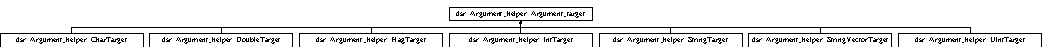
\includegraphics[height=0.629921cm]{classdsr_1_1_argument__helper_1_1_argument__target}
\end{center}
\end{figure}
\subsection*{Public Member Functions}
\begin{DoxyCompactItemize}
\item 
\hypertarget{classdsr_1_1_argument__helper_1_1_argument__target_a18fa4db232e09c250726f6205d4ed46f}{
{\bfseries Argument\_\-target} (char k, const std::string lname, const std::string descr, const std::string arg\_\-descr)}
\label{classdsr_1_1_argument__helper_1_1_argument__target_a18fa4db232e09c250726f6205d4ed46f}

\item 
\hypertarget{classdsr_1_1_argument__helper_1_1_argument__target_a7f94fa839300ae7b11a785c2548635f5}{
{\bfseries Argument\_\-target} (const std::string descr, const std::string arg\_\-descr)}
\label{classdsr_1_1_argument__helper_1_1_argument__target_a7f94fa839300ae7b11a785c2548635f5}

\item 
\hypertarget{classdsr_1_1_argument__helper_1_1_argument__target_a4892e51b63fba18bbb0a562b48048340}{
virtual bool {\bfseries process} (int \&, const char $\ast$$\ast$\&)=0}
\label{classdsr_1_1_argument__helper_1_1_argument__target_a4892e51b63fba18bbb0a562b48048340}

\item 
\hypertarget{classdsr_1_1_argument__helper_1_1_argument__target_a3d4e24d28b68d7077caaec7af840ba65}{
virtual void {\bfseries write\_\-name} (std::ostream \&out) const }
\label{classdsr_1_1_argument__helper_1_1_argument__target_a3d4e24d28b68d7077caaec7af840ba65}

\item 
\hypertarget{classdsr_1_1_argument__helper_1_1_argument__target_a07b67b02d88b4db5cf6aef6bcca7d344}{
virtual void {\bfseries write\_\-value} (std::ostream \&out) const =0}
\label{classdsr_1_1_argument__helper_1_1_argument__target_a07b67b02d88b4db5cf6aef6bcca7d344}

\item 
\hypertarget{classdsr_1_1_argument__helper_1_1_argument__target_aed6a18e0271c428a3d6edd4e0a45455f}{
virtual void {\bfseries write\_\-usage} (std::ostream \&out) const }
\label{classdsr_1_1_argument__helper_1_1_argument__target_aed6a18e0271c428a3d6edd4e0a45455f}

\end{DoxyCompactItemize}
\subsection*{Public Attributes}
\begin{DoxyCompactItemize}
\item 
\hypertarget{classdsr_1_1_argument__helper_1_1_argument__target_a3cc92480d2fcb208164e63907cb6e87e}{
char {\bfseries key}}
\label{classdsr_1_1_argument__helper_1_1_argument__target_a3cc92480d2fcb208164e63907cb6e87e}

\item 
\hypertarget{classdsr_1_1_argument__helper_1_1_argument__target_a6aa32e96af30ba3e4139876c07af96b2}{
std::string {\bfseries long\_\-name}}
\label{classdsr_1_1_argument__helper_1_1_argument__target_a6aa32e96af30ba3e4139876c07af96b2}

\item 
\hypertarget{classdsr_1_1_argument__helper_1_1_argument__target_a0ff169144da0b246ecf6d8980d60a7b1}{
std::string {\bfseries description}}
\label{classdsr_1_1_argument__helper_1_1_argument__target_a0ff169144da0b246ecf6d8980d60a7b1}

\item 
\hypertarget{classdsr_1_1_argument__helper_1_1_argument__target_afef131ac78b225c4f008264c3e50e23b}{
std::string {\bfseries arg\_\-description}}
\label{classdsr_1_1_argument__helper_1_1_argument__target_afef131ac78b225c4f008264c3e50e23b}

\end{DoxyCompactItemize}


The documentation for this class was generated from the following file:\begin{DoxyCompactItemize}
\item 
Argument\_\-helper.cpp\end{DoxyCompactItemize}

\hypertarget{classdsr_1_1_argument__helper_1_1_char_target}{
\section{dsr::Argument\_\-helper::CharTarget Class Reference}
\label{classdsr_1_1_argument__helper_1_1_char_target}\index{dsr::Argument\_\-helper::CharTarget@{dsr::Argument\_\-helper::CharTarget}}
}
Inheritance diagram for dsr::Argument\_\-helper::CharTarget:\begin{figure}[H]
\begin{center}
\leavevmode
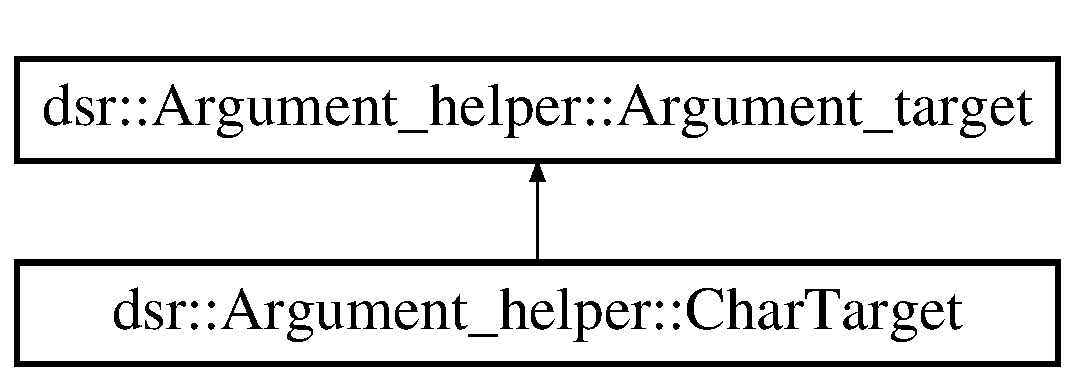
\includegraphics[height=2.000000cm]{classdsr_1_1_argument__helper_1_1_char_target}
\end{center}
\end{figure}
\subsection*{Public Member Functions}
\begin{DoxyCompactItemize}
\item 
\hypertarget{classdsr_1_1_argument__helper_1_1_char_target_a67e0d2c68b25ac08847ddcff8f83f626}{
{\bfseries CharTarget} (char k, const char $\ast$lname, const char $\ast$arg\_\-descr, const char $\ast$descr, char \&b)}
\label{classdsr_1_1_argument__helper_1_1_char_target_a67e0d2c68b25ac08847ddcff8f83f626}

\item 
\hypertarget{classdsr_1_1_argument__helper_1_1_char_target_ad5bb65eb61f4401f4b166b3bd6f9a0c3}{
{\bfseries CharTarget} (const char $\ast$arg\_\-descr, const char $\ast$descr, char \&b)}
\label{classdsr_1_1_argument__helper_1_1_char_target_ad5bb65eb61f4401f4b166b3bd6f9a0c3}

\item 
\hypertarget{classdsr_1_1_argument__helper_1_1_char_target_ac8a645a4a92249301251a8b4df20c7de}{
virtual bool {\bfseries process} (int \&argc, const char $\ast$$\ast$\&argv)}
\label{classdsr_1_1_argument__helper_1_1_char_target_ac8a645a4a92249301251a8b4df20c7de}

\item 
\hypertarget{classdsr_1_1_argument__helper_1_1_char_target_a911c060da0c153e07dbd0241441e3fc0}{
virtual void {\bfseries write\_\-value} (std::ostream \&out) const }
\label{classdsr_1_1_argument__helper_1_1_char_target_a911c060da0c153e07dbd0241441e3fc0}

\end{DoxyCompactItemize}
\subsection*{Public Attributes}
\begin{DoxyCompactItemize}
\item 
\hypertarget{classdsr_1_1_argument__helper_1_1_char_target_af5c1784371ae17cb26c1a4ea12ff762b}{
char \& {\bfseries val}}
\label{classdsr_1_1_argument__helper_1_1_char_target_af5c1784371ae17cb26c1a4ea12ff762b}

\end{DoxyCompactItemize}


The documentation for this class was generated from the following file:\begin{DoxyCompactItemize}
\item 
Argument\_\-helper.cpp\end{DoxyCompactItemize}

\hypertarget{classdsr_1_1_argument__helper_1_1_double_target}{
\section{dsr::Argument\_\-helper::DoubleTarget Class Reference}
\label{classdsr_1_1_argument__helper_1_1_double_target}\index{dsr::Argument\_\-helper::DoubleTarget@{dsr::Argument\_\-helper::DoubleTarget}}
}
Inheritance diagram for dsr::Argument\_\-helper::DoubleTarget:\begin{figure}[H]
\begin{center}
\leavevmode
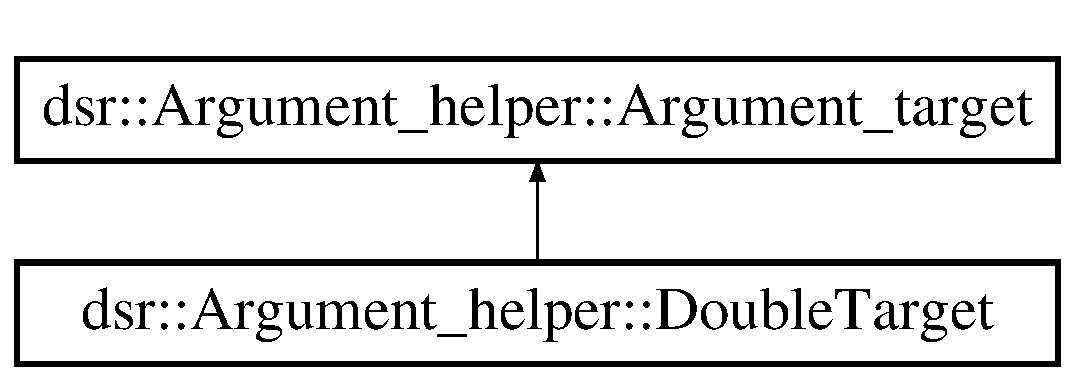
\includegraphics[height=2.000000cm]{classdsr_1_1_argument__helper_1_1_double_target}
\end{center}
\end{figure}
\subsection*{Public Member Functions}
\begin{DoxyCompactItemize}
\item 
\hypertarget{classdsr_1_1_argument__helper_1_1_double_target_aed3e046727cba857a4b59a1a9a08bed3}{
{\bfseries DoubleTarget} (char k, const char $\ast$lname, const char $\ast$arg\_\-descr, const char $\ast$descr, double \&b)}
\label{classdsr_1_1_argument__helper_1_1_double_target_aed3e046727cba857a4b59a1a9a08bed3}

\item 
\hypertarget{classdsr_1_1_argument__helper_1_1_double_target_a4cd0b54e751663b37ba61bb307ac1e63}{
{\bfseries DoubleTarget} (const char $\ast$arg\_\-descr, const char $\ast$descr, double \&b)}
\label{classdsr_1_1_argument__helper_1_1_double_target_a4cd0b54e751663b37ba61bb307ac1e63}

\item 
\hypertarget{classdsr_1_1_argument__helper_1_1_double_target_a46f012c8675d9c5b0edb08376e7184e2}{
virtual bool {\bfseries process} (int \&argc, const char $\ast$$\ast$\&argv)}
\label{classdsr_1_1_argument__helper_1_1_double_target_a46f012c8675d9c5b0edb08376e7184e2}

\item 
\hypertarget{classdsr_1_1_argument__helper_1_1_double_target_a18f128db07755a735f800dea569131f0}{
virtual void {\bfseries write\_\-value} (std::ostream \&out) const }
\label{classdsr_1_1_argument__helper_1_1_double_target_a18f128db07755a735f800dea569131f0}

\end{DoxyCompactItemize}
\subsection*{Public Attributes}
\begin{DoxyCompactItemize}
\item 
\hypertarget{classdsr_1_1_argument__helper_1_1_double_target_a4125e3b92cebd0add6c62428266caace}{
double \& {\bfseries val}}
\label{classdsr_1_1_argument__helper_1_1_double_target_a4125e3b92cebd0add6c62428266caace}

\end{DoxyCompactItemize}


The documentation for this class was generated from the following file:\begin{DoxyCompactItemize}
\item 
Argument\_\-helper.cpp\end{DoxyCompactItemize}

\hypertarget{classdsr_1_1_argument__helper_1_1_flag_target}{
\section{dsr::Argument\_\-helper::FlagTarget Class Reference}
\label{classdsr_1_1_argument__helper_1_1_flag_target}\index{dsr::Argument\_\-helper::FlagTarget@{dsr::Argument\_\-helper::FlagTarget}}
}
Inheritance diagram for dsr::Argument\_\-helper::FlagTarget:\begin{figure}[H]
\begin{center}
\leavevmode
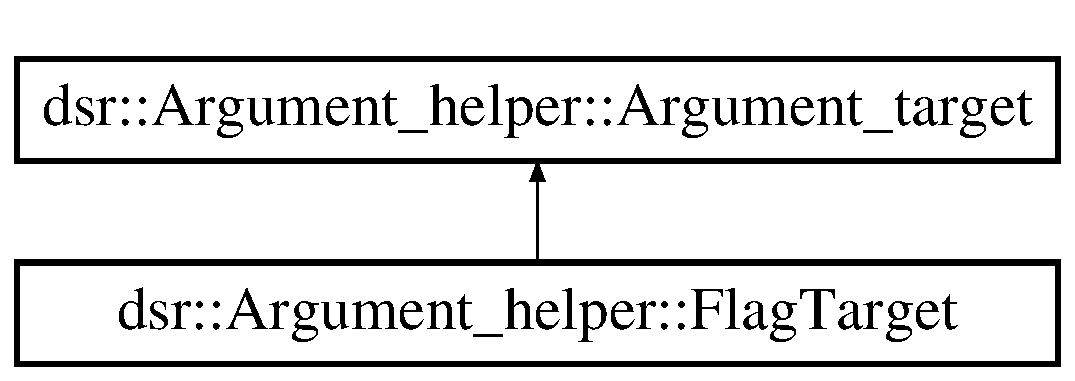
\includegraphics[height=2.000000cm]{classdsr_1_1_argument__helper_1_1_flag_target}
\end{center}
\end{figure}
\subsection*{Public Member Functions}
\begin{DoxyCompactItemize}
\item 
\hypertarget{classdsr_1_1_argument__helper_1_1_flag_target_ae7389f3d11744d5f5dc30632f8f393cc}{
{\bfseries FlagTarget} (char k, const char $\ast$lname, const char $\ast$descr, bool \&b)}
\label{classdsr_1_1_argument__helper_1_1_flag_target_ae7389f3d11744d5f5dc30632f8f393cc}

\item 
\hypertarget{classdsr_1_1_argument__helper_1_1_flag_target_a9fe646d89cb09d86d0d95bd6d018b778}{
virtual bool {\bfseries process} (int \&, const char $\ast$$\ast$\&)}
\label{classdsr_1_1_argument__helper_1_1_flag_target_a9fe646d89cb09d86d0d95bd6d018b778}

\item 
\hypertarget{classdsr_1_1_argument__helper_1_1_flag_target_ae1ca137885097714ad4a7cc13d477e64}{
virtual void {\bfseries write\_\-value} (std::ostream \&out) const }
\label{classdsr_1_1_argument__helper_1_1_flag_target_ae1ca137885097714ad4a7cc13d477e64}

\item 
\hypertarget{classdsr_1_1_argument__helper_1_1_flag_target_a26dcc0b9897f36d961367c86911a550d}{
virtual void {\bfseries write\_\-usage} (std::ostream \&out) const }
\label{classdsr_1_1_argument__helper_1_1_flag_target_a26dcc0b9897f36d961367c86911a550d}

\end{DoxyCompactItemize}
\subsection*{Public Attributes}
\begin{DoxyCompactItemize}
\item 
\hypertarget{classdsr_1_1_argument__helper_1_1_flag_target_a7671d7ad6767cf131f5d456b892b0a80}{
bool \& {\bfseries val}}
\label{classdsr_1_1_argument__helper_1_1_flag_target_a7671d7ad6767cf131f5d456b892b0a80}

\end{DoxyCompactItemize}


The documentation for this class was generated from the following file:\begin{DoxyCompactItemize}
\item 
Argument\_\-helper.cpp\end{DoxyCompactItemize}

\hypertarget{classdsr_1_1_argument__helper_1_1_int_target}{
\section{dsr::Argument\_\-helper::IntTarget Class Reference}
\label{classdsr_1_1_argument__helper_1_1_int_target}\index{dsr::Argument\_\-helper::IntTarget@{dsr::Argument\_\-helper::IntTarget}}
}
Inheritance diagram for dsr::Argument\_\-helper::IntTarget:\begin{figure}[H]
\begin{center}
\leavevmode
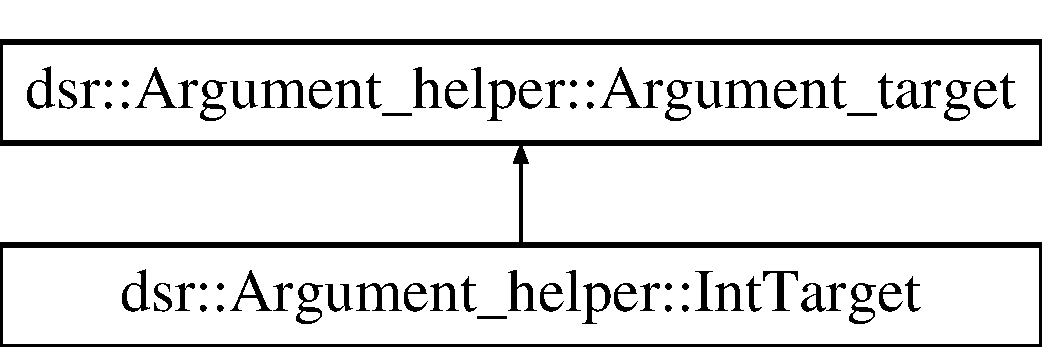
\includegraphics[height=2.000000cm]{classdsr_1_1_argument__helper_1_1_int_target}
\end{center}
\end{figure}
\subsection*{Public Member Functions}
\begin{DoxyCompactItemize}
\item 
\hypertarget{classdsr_1_1_argument__helper_1_1_int_target_a1171f49a361db468253da0c5a900e2b6}{
{\bfseries IntTarget} (const char $\ast$arg\_\-descr, const char $\ast$descr, int \&b)}
\label{classdsr_1_1_argument__helper_1_1_int_target_a1171f49a361db468253da0c5a900e2b6}

\item 
\hypertarget{classdsr_1_1_argument__helper_1_1_int_target_a3efaed5093d6c20bcf65ea19edcff2bb}{
{\bfseries IntTarget} (char k, const char $\ast$lname, const char $\ast$arg\_\-descr, const char $\ast$descr, int \&b)}
\label{classdsr_1_1_argument__helper_1_1_int_target_a3efaed5093d6c20bcf65ea19edcff2bb}

\item 
\hypertarget{classdsr_1_1_argument__helper_1_1_int_target_a83b77c377f15298ff2d2149c1e460004}{
virtual bool {\bfseries process} (int \&argc, const char $\ast$$\ast$\&argv)}
\label{classdsr_1_1_argument__helper_1_1_int_target_a83b77c377f15298ff2d2149c1e460004}

\item 
\hypertarget{classdsr_1_1_argument__helper_1_1_int_target_a7d2d812aa5a2b6530ca69ebb12b7541d}{
virtual void {\bfseries write\_\-value} (std::ostream \&out) const }
\label{classdsr_1_1_argument__helper_1_1_int_target_a7d2d812aa5a2b6530ca69ebb12b7541d}

\end{DoxyCompactItemize}
\subsection*{Public Attributes}
\begin{DoxyCompactItemize}
\item 
\hypertarget{classdsr_1_1_argument__helper_1_1_int_target_a36998950d2fcfd87c92573d3f8706852}{
int \& {\bfseries val}}
\label{classdsr_1_1_argument__helper_1_1_int_target_a36998950d2fcfd87c92573d3f8706852}

\end{DoxyCompactItemize}


The documentation for this class was generated from the following file:\begin{DoxyCompactItemize}
\item 
Argument\_\-helper.cpp\end{DoxyCompactItemize}

\hypertarget{classdsr_1_1_argument__helper_1_1_string_target}{
\section{dsr::Argument\_\-helper::StringTarget Class Reference}
\label{classdsr_1_1_argument__helper_1_1_string_target}\index{dsr::Argument\_\-helper::StringTarget@{dsr::Argument\_\-helper::StringTarget}}
}
Inheritance diagram for dsr::Argument\_\-helper::StringTarget:\begin{figure}[H]
\begin{center}
\leavevmode
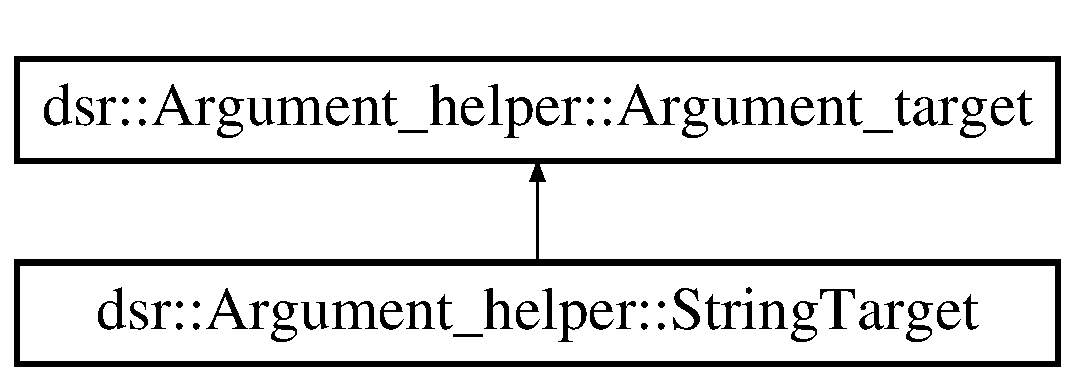
\includegraphics[height=2.000000cm]{classdsr_1_1_argument__helper_1_1_string_target}
\end{center}
\end{figure}
\subsection*{Public Member Functions}
\begin{DoxyCompactItemize}
\item 
\hypertarget{classdsr_1_1_argument__helper_1_1_string_target_abbaf278629fe7019d9dd5018ab544b64}{
{\bfseries StringTarget} (const char $\ast$arg\_\-descr, const char $\ast$descr, std::string \&b)}
\label{classdsr_1_1_argument__helper_1_1_string_target_abbaf278629fe7019d9dd5018ab544b64}

\item 
\hypertarget{classdsr_1_1_argument__helper_1_1_string_target_a3528a449e48433bc0fab249a02913d8d}{
{\bfseries StringTarget} (char k, const char $\ast$lname, const char $\ast$arg\_\-descr, const char $\ast$descr, std::string \&b)}
\label{classdsr_1_1_argument__helper_1_1_string_target_a3528a449e48433bc0fab249a02913d8d}

\item 
\hypertarget{classdsr_1_1_argument__helper_1_1_string_target_a38a81be4a7d8bf51eefbeb7bd7f38bea}{
virtual bool {\bfseries process} (int \&argc, const char $\ast$$\ast$\&argv)}
\label{classdsr_1_1_argument__helper_1_1_string_target_a38a81be4a7d8bf51eefbeb7bd7f38bea}

\item 
\hypertarget{classdsr_1_1_argument__helper_1_1_string_target_a083f06031c7f4a9408d0ebb7f3a21352}{
virtual void {\bfseries write\_\-value} (std::ostream \&out) const }
\label{classdsr_1_1_argument__helper_1_1_string_target_a083f06031c7f4a9408d0ebb7f3a21352}

\end{DoxyCompactItemize}
\subsection*{Public Attributes}
\begin{DoxyCompactItemize}
\item 
\hypertarget{classdsr_1_1_argument__helper_1_1_string_target_a07497eff5e99993cf79865284610c6e1}{
std::string \& {\bfseries val}}
\label{classdsr_1_1_argument__helper_1_1_string_target_a07497eff5e99993cf79865284610c6e1}

\end{DoxyCompactItemize}


The documentation for this class was generated from the following file:\begin{DoxyCompactItemize}
\item 
Argument\_\-helper.cpp\end{DoxyCompactItemize}

\hypertarget{classdsr_1_1_argument__helper_1_1_string_vector_target}{
\section{dsr::Argument\_\-helper::StringVectorTarget Class Reference}
\label{classdsr_1_1_argument__helper_1_1_string_vector_target}\index{dsr::Argument\_\-helper::StringVectorTarget@{dsr::Argument\_\-helper::StringVectorTarget}}
}
Inheritance diagram for dsr::Argument\_\-helper::StringVectorTarget:\begin{figure}[H]
\begin{center}
\leavevmode
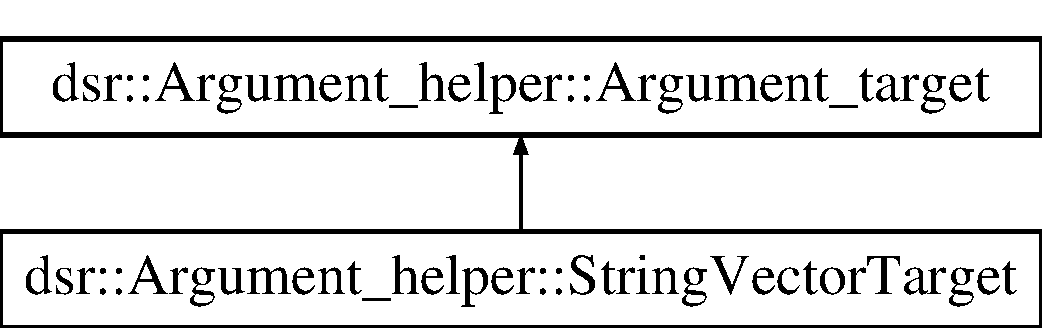
\includegraphics[height=2.000000cm]{classdsr_1_1_argument__helper_1_1_string_vector_target}
\end{center}
\end{figure}
\subsection*{Public Member Functions}
\begin{DoxyCompactItemize}
\item 
\hypertarget{classdsr_1_1_argument__helper_1_1_string_vector_target_a895759376a79e9cc282783a3a5be7cc7}{
{\bfseries StringVectorTarget} (char k, const char $\ast$lname, const char $\ast$arg\_\-descr, const char $\ast$descr, std::vector$<$ std::string $>$ \&b)}
\label{classdsr_1_1_argument__helper_1_1_string_vector_target_a895759376a79e9cc282783a3a5be7cc7}

\item 
\hypertarget{classdsr_1_1_argument__helper_1_1_string_vector_target_a711141af8e59f26e382f8ce6b5791d61}{
virtual bool {\bfseries process} (int \&argc, const char $\ast$$\ast$\&argv)}
\label{classdsr_1_1_argument__helper_1_1_string_vector_target_a711141af8e59f26e382f8ce6b5791d61}

\item 
\hypertarget{classdsr_1_1_argument__helper_1_1_string_vector_target_a85cc5e5007041c129d674e8fda98f6db}{
virtual void {\bfseries write\_\-value} (std::ostream \&out) const }
\label{classdsr_1_1_argument__helper_1_1_string_vector_target_a85cc5e5007041c129d674e8fda98f6db}

\end{DoxyCompactItemize}
\subsection*{Public Attributes}
\begin{DoxyCompactItemize}
\item 
\hypertarget{classdsr_1_1_argument__helper_1_1_string_vector_target_a4fb78576f9c6adc639202d560493808c}{
std::vector$<$ std::string $>$ \& {\bfseries val}}
\label{classdsr_1_1_argument__helper_1_1_string_vector_target_a4fb78576f9c6adc639202d560493808c}

\end{DoxyCompactItemize}


The documentation for this class was generated from the following file:\begin{DoxyCompactItemize}
\item 
Argument\_\-helper.cpp\end{DoxyCompactItemize}

\hypertarget{classdsr_1_1_argument__helper_1_1_u_int_target}{
\section{dsr::Argument\_\-helper::UIntTarget Class Reference}
\label{classdsr_1_1_argument__helper_1_1_u_int_target}\index{dsr::Argument\_\-helper::UIntTarget@{dsr::Argument\_\-helper::UIntTarget}}
}
Inheritance diagram for dsr::Argument\_\-helper::UIntTarget:\begin{figure}[H]
\begin{center}
\leavevmode
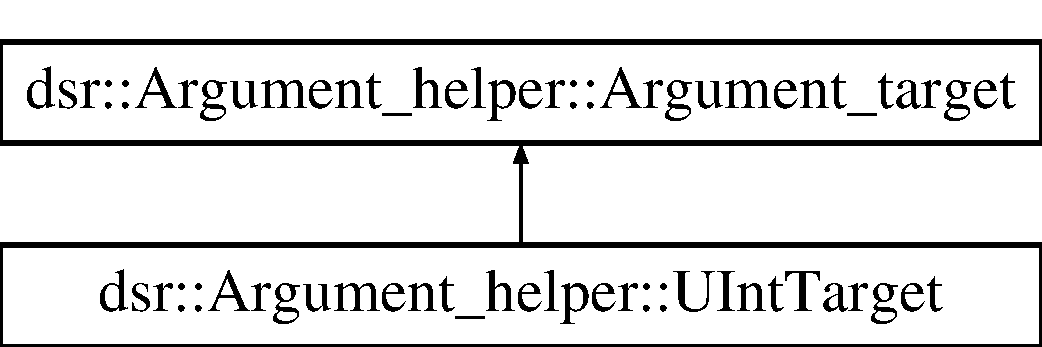
\includegraphics[height=2.000000cm]{classdsr_1_1_argument__helper_1_1_u_int_target}
\end{center}
\end{figure}
\subsection*{Public Member Functions}
\begin{DoxyCompactItemize}
\item 
\hypertarget{classdsr_1_1_argument__helper_1_1_u_int_target_a3d9454fceac68d4271b3127a9846e38d}{
{\bfseries UIntTarget} (const char $\ast$arg\_\-descr, const char $\ast$descr, unsigned int \&b)}
\label{classdsr_1_1_argument__helper_1_1_u_int_target_a3d9454fceac68d4271b3127a9846e38d}

\item 
\hypertarget{classdsr_1_1_argument__helper_1_1_u_int_target_a65b049d566055fa7086be18a083a22f3}{
{\bfseries UIntTarget} (char k, const char $\ast$lname, const char $\ast$arg\_\-descr, const char $\ast$descr, unsigned int \&b)}
\label{classdsr_1_1_argument__helper_1_1_u_int_target_a65b049d566055fa7086be18a083a22f3}

\item 
\hypertarget{classdsr_1_1_argument__helper_1_1_u_int_target_a6ef1c90bb75d83f03adcf17b823509f5}{
virtual bool {\bfseries process} (int \&argc, const char $\ast$$\ast$\&argv)}
\label{classdsr_1_1_argument__helper_1_1_u_int_target_a6ef1c90bb75d83f03adcf17b823509f5}

\item 
\hypertarget{classdsr_1_1_argument__helper_1_1_u_int_target_aab39ece4f7160e8b74ca324505acc3ed}{
virtual void {\bfseries write\_\-value} (std::ostream \&out) const }
\label{classdsr_1_1_argument__helper_1_1_u_int_target_aab39ece4f7160e8b74ca324505acc3ed}

\end{DoxyCompactItemize}
\subsection*{Public Attributes}
\begin{DoxyCompactItemize}
\item 
\hypertarget{classdsr_1_1_argument__helper_1_1_u_int_target_a67d64513611e9c34d4b64ff021338878}{
unsigned int \& {\bfseries val}}
\label{classdsr_1_1_argument__helper_1_1_u_int_target_a67d64513611e9c34d4b64ff021338878}

\end{DoxyCompactItemize}


The documentation for this class was generated from the following file:\begin{DoxyCompactItemize}
\item 
Argument\_\-helper.cpp\end{DoxyCompactItemize}

\printindex
\end{document}
